% =============================================================================
% CHAPTER ONE - INTRODUCTION
%
% Structure follows Appendix III A of the UB guide (applied sciences):
%   1.1 Background to the study
%   1.2 Problem statement
%   1.3 Rationale of the study
%   1.4 Objectives and hypotheses
% plus the customary engineering additions (research questions, scope,
% significance, definition of terms, organisation of the thesis).
%
% House rules for this file:
%   * No em dashes. Use commas, colons, semicolons or parentheses.
%   * No vertical space between paragraphs; first-line indent separates them.
%   * Every claim carries a citation or is marked %% VERIFY.
%
% STATUS: fourth draft (v4). See thesis/JOURNAL.md.
%   * State things directly. No meta-commentary about method or framework.
% =============================================================================

\chapter{Introduction}
\label{ch:introduction}

\section{Background to the Study}
\label{sec:background}

Agriculture is undergoing a transition from experience-driven practice to
data-driven decision making. Networks of low-cost sensors now measure soil
moisture, canopy temperature, humidity and nutrient status continuously, and
the resulting streams feed irrigation controllers, yield models and
certification schemes~\cite{rathi2025smart, brooks2019precisionWater}. In
water-stressed regions this shift is not a convenience but a necessity.
Irrigation accounts for the dominant share of freshwater withdrawal, and
climate variability has compressed the margin for error in scheduling
decisions~\cite{miller2020climateImpact, williams2022savings}.

A measurement taken in a field does not stop at the field. It becomes a record,
and that record is consumed by parties with interests of their own, as
Figure~\ref{fig:lifecycle} sets out. The value of the record to those parties
is exactly what creates the incentive to falsify it, and the further a record
travels from the instrument that produced it, the weaker the evidence that it
is genuine.

\begin{figure}[htbp]
  \centering
  \begin{tikzpicture}[
      box/.style={draw, rounded corners=2pt, align=center, font=\small,
                  minimum height=9mm, inner sep=4pt},
      use/.style={box, fill=black!4, text width=26mm},
      flow/.style={-{Stealth[length=2mm]}, thick},
      note/.style={font=\footnotesize\itshape, align=center, text width=90mm}
    ]
    \node[box, text width=23mm] (field)  at (0,0)      {Field\\measurement};
    \node[box, text width=23mm] (record) at (3.7,0)    {Agricultural\\record};

    \node[use] (cert) at (8.0, 1.5)  {Certification\\(organic, fair trade)};
    \node[use] (ins)  at (8.0, 0)    {Index-based\\crop insurance};
    \node[use] (sub)  at (8.0,-1.5)  {Subsidy\\allocation};

    \draw[flow] (field) -- (record);
    \draw[flow] (record.east) -- (cert.west);
    \draw[flow] (record.east) -- (ins.west);
    \draw[flow] (record.east) -- (sub.west);

    % No leader line: it would cross the note text. Position carries the
    % association well enough.
    \node[note] (inc) at (4.0,-2.9)
      {Each downstream use attaches value to the record,\\
       and therefore creates an incentive to falsify it.};
  \end{tikzpicture}
  \caption{Lifecycle of an agricultural measurement: a reading becomes a
           record whose downstream value creates the incentive to falsify it.}
  \label{fig:lifecycle}
\end{figure}

Reviews of the sensing layer converge on the same reading. Smart sensing has
matured to the point where measurement is no longer the constraint, while the
integration of that measurement into auditable decision-making
remains~\cite{soussi2024smartsensors, gong2025edge}. Surveys of edge-enabled
agriculture name communication reliability and energy constraints as the two
bottlenecks that most often defeat field deployments~\cite{gong2025edge}, and
surveys of the wider \gls{iot} threat surface agree that the constrained
endpoint is the weakest link in the provenance chain~\cite{aouedi2024surveyintelligent, sahu2024exploringsecurity}.

The economics of the sensing layer explain why the problem is hard rather than
merely tedious. A deployment that is worth installing on a smallholding must
cost a small fraction of the crop value it protects, which forces the node bill
of materials down to a level at which neither a hardware security module nor a
generous energy budget is affordable. The same economics rule out mains power
and wired backhaul across a field, so the design space collapses onto
battery-powered microcontrollers speaking a long-range, low-rate radio. Every
protection mechanism proposed in this thesis has to survive inside that
envelope, and a mechanism that works only on a mains-powered gateway has solved
the easier half of the problem.

The sensing layer of such systems is built from severely constrained devices.
An \gls{esp32} node operating on battery and harvested solar power must
transmit over kilometre-scale distances using \gls{lora}, a modulation scheme
that trades data rate for range and therefore charges a high airtime cost per
packet~\cite{raza2018lorawan, adelantado2017understanding}. Airtime is the
binding constraint. It determines energy consumption at the node, and, through
duty-cycle regulation and collision probability, it determines how many nodes a
single gateway can serve~\cite{mohammed2025loraEnergy}. Conventional responses
compress the payload, but general-purpose compressors such as Huffman and
\gls{lzw} carry dictionary and buffer overheads that a microcontroller with a
few kilobytes of free \gls{ram} can ill
afford~\cite{marcelloni2009energy, chen2025compression}.

Two further constraints sharpen this. Sub-GHz \gls{iot} bands are governed by a
duty-cycle limit, so a node that has just transmitted must stay silent for a
period proportional to the airtime it consumed. Airtime is therefore not only
an energy cost but a rate limit: it caps how often a node may report, and no
increase in battery capacity relaxes it. Second, because \gls{lora} uses
unslotted access, packets collide whenever two nodes transmit on the same
channel at the same time, and the collision probability grows with the square
of offered traffic in the regime that matters. Halving per-packet occupancy
therefore buys more than a proportional reduction in collisions, which is why
the mechanism studied here is worth the arithmetic it costs. Figure~\ref{fig:airtime-chain}
sets out how one quantity, airtime per packet, propagates into three
consequences that a design cannot address independently.

\begin{figure}[htbp]
  \centering
  \begin{tikzpicture}[
      box/.style={draw, rounded corners=2pt, align=center, font=\small,
                  minimum height=9mm, inner sep=4pt},
      src/.style={box, fill=black!4, text width=28mm},
      mid/.style={box, fill=black!4, text width=30mm},
      res/.style={box, fill=black!8, text width=30mm, font=\small\bfseries},
      flow/.style={-{Stealth[length=2mm]}, thick},
      note/.style={font=\footnotesize\itshape, align=center, text width=115mm}
    ]
    \node[src] (payload)  at (0,3.4)   {Per-packet\\payload size};
    \node[src, text width=32mm] (airtime) at (5.2,3.4) {Airtime spent\\per packet};

    \node[mid] (energy) at (-3.2,0.8) {Energy drawn\\from the battery};
    \node[mid] (duty)   at (2.2,0.8)  {Mandatory\\silence period};
    \node[mid] (coll)   at (7.6,0.8)  {Collision\\probability};

    \node[res] (battery)  at (-3.2,-1.7) {Battery\\lifetime};
    \node[res] (capacity) at (4.9,-1.7)  {Gateway packet\\capacity};

    \draw[flow] (payload) -- (airtime);
    \draw[flow] (airtime.south) -- ++(0,-0.5) -| (energy.north);
    \draw[flow] (airtime.south) -- ++(0,-0.5) -| (duty.north);
    \draw[flow] (airtime.south) -- ++(0,-0.5) -| (coll.north);

    \draw[flow] (energy) -- (battery);
    \draw[flow] (duty)   -- (capacity);
    \draw[flow] (coll)   -- (capacity);

    \node[note] at (2.2,-3.4)
      {A shorter payload lowers airtime once, and that single reduction pays
       three times: less energy drawn per reading, a shorter mandatory
       silence period, and a lower collision probability at the gateway.};
  \end{tikzpicture}
  \caption{Airtime is a rate limit, not only an energy cost: reducing it
           relaxes the duty-cycle and collision ceilings on gateway capacity.}
  \label{fig:airtime-chain}
\end{figure}

The \gls{crt} offers a different route. Decomposing a reading into residues
modulo pairwise coprime moduli yields several short packets in place of one
long one~\cite{garner1959residue, ding1996remainder}. Because a multi-channel
concentrator such as the SX1302 demodulates channels concurrently, the short
residue packets can be received simultaneously, and the original value is
recovered in $O(k)$ operations for $k$ moduli. The practical effect is a
reduction in per-packet occupancy rather than in total transmitted volume,
which is precisely the quantity that governs gateway capacity. The detailed
encoding and reconstruction path is presented in Chapter Three.

Residue arithmetic is not new to distributed systems. The same decomposition
underlies the throughput work in permissionless ledgers, where partitioning a
workload across independent classes lets operations commit concurrently that
would otherwise serialise~\cite{maiwada2025blockchainscalability, maiwada2024techniquesimprove, horvath2025assistedsharding}, and the algebraic
machinery itself has been carried well beyond integer
congruences~\cite{luo2023researchapplication}. That line of work establishes
the arithmetic and the parallelisation argument. What it does not address is
the constrained radio link, where the payoff is airtime rather than processor
cycles, nor the identity and confidentiality questions that arise when the
residues cross a shared medium. A single result hints that the second is
reachable: residue decomposition combined with chaotic maps has been used to
conceal image content reversibly~\cite{yavuz2025reversibledata}, which suggests
residues can carry confidentiality as well as efficiency, albeit under a
different medium and threat model. This thesis takes the arithmetic as
established and asks what it is worth on the edge of the network rather than at
its centre~\cite{forcha2026basedparallel}.

Data that has been collected cheaply must then be trusted. Agricultural records
increasingly carry consequences beyond the farm gate. They substantiate organic
and fair-trade certification, they underwrite index-based crop insurance, and
they inform subsidy allocation. Each of these uses creates an incentive to
falsify. A centralised database concentrates that risk in a single
administrator, and an unprotected sensor network invites the injection of
fabricated readings by any party with a compatible radio. \gls{dlt} addresses
the tamper-evidence requirement by binding records into a hash-linked chain
replicated across mutually distrusting parties, and permissioned platforms such
as \gls{hlf} add an identity layer through a \gls{msp} and \gls{pki}, making it
feasible to say not merely that a record is unaltered but who produced
it~\cite{tar2023fabric, jayaram2023hyperledger, dube2024fabricIrrigation}.

Running that machinery at the edge is the difficulty. Consensus, endorsement and
world-state maintenance were designed for datacentre hardware, whereas an
agricultural deployment must place gateways in the field, on \gls{arm64}
single-board computers, behind intermittent connectivity. Whether a permissioned
ledger can meet irrigation-control timing requirements on such hardware has
until recently been asserted rather than measured.

Finally, protection is not exhausted by integrity. A soil-moisture trace is also
a disclosure. It reveals plot productivity, irrigation strategy and, in
aggregate, the commercial position of the farmer. Where records are replicated
across a consortium that includes buyers, insurers and cooperatives, the same
replication that secures integrity enlarges the audience for private
information. Identity, integrity and privacy therefore have to be treated as one
design problem rather than three independent ones, which is the position this
thesis takes.

\section{Statement of the Problem}
\label{sec:problem}

Three properties that ought to hold simultaneously are, in current systems,
traded against one another.

\textbf{Identity is weak at the sensing layer.} Constrained nodes seldom carry
credentials strong enough to authenticate individual readings. Where
authentication exists it typically terminates at the gateway, so the ledger
attests to what the gateway submitted rather than to what the sensor measured.
The provenance chain has a gap exactly where falsification is cheapest, at the
final hop between an individual node and the record that claims to represent
it.

Farm-specific work confirms that the exposure is real rather than theoretical.
Tampering with \gls{iot} farm data has been treated as a distinct security
problem requiring its own countermeasures~\cite{ali2023farmDataTampering}, and
production deployments in food chains report provenance as the primary
motivation for adopting a ledger at all~\cite{safeer2024tomato, tang2025applicationsblockchain}.

\textbf{Integrity guarantees do not survive the move to the edge.} Permissioned
ledgers provide tamper evidence, but their published performance
characterisations assume server-class hosts. On \gls{arm64} gateways with
constrained memory and intermittent links, it is not established that
endorsement and ordering can complete inside the control loop of an irrigation
decision, nor how the ledger behaves during network partition and recovery.

\textbf{Privacy is sacrificed to obtain integrity.} Replicating raw agronomic
readings to every consortium member is the simplest way to make them verifiable
and the worst way to keep them confidential. Existing deployments largely accept
this trade, or push confidential data off chain in a way that reintroduces the
trusted intermediary the ledger was meant to remove.

The three shortfalls, shown together in Figure~\ref{fig:three-properties}, are
not independent faults to be repaired one at a time. Each follows from the same
scarcity, and a remedy applied to one is paid for out of the budget available
to the others.

\begin{figure}[htbp]
  \centering
  \begin{tikzpicture}[
      prop/.style={draw, thick, rounded corners=2pt, align=center,
                   font=\small\bfseries, minimum height=8mm, inner sep=4pt,
                   fill=white},
      gap/.style={font=\footnotesize\itshape, align=center, text width=34mm},
      link/.style={{Stealth[length=2mm]}-{Stealth[length=2mm]}, gray, thin}
    ]
    \node[prop] (id)  at (0,2.5)   {Identity};
    \node[prop] (int) at (-3.2,0)  {Integrity};
    \node[prop] (pri) at (3.2,0)   {Privacy};

    \draw[link] (id)  -- (int);
    \draw[link] (int) -- (pri);
    \draw[link] (pri) -- (id);

    % Annotations sit inside the boundary, never across it.
    \node[gap] (gid)  at (0,3.5)     {authentication stops\\at the gateway};
    \node[gap] (gint) at (-3.2,-1.1) {ledger cost unproven\\on edge hardware};
    \node[gap] (gpri) at (3.2,-1.1)  {confidentiality traded\\away for verifiability};

    \begin{scope}[on background layer]
      \node[draw, dashed, thick, rounded corners=4pt, fill=black!3,
            fit=(id)(int)(pri)(gid)(gint)(gpri), inner sep=5mm] (budget) {};
    \end{scope}
    \node[font=\small\itshape, below=1.5mm of budget.south]
      {bounded by one shared energy, memory and channel budget};
  \end{tikzpicture}
  \caption{The three protection properties, sharing one constrained budget
           and therefore one design problem.}
  \label{fig:three-properties}
\end{figure}

Underlying all three is a resource problem. The transmission budget that would
pay for per-reading signatures, encryption and privacy-preserving encodings is
already consumed by the raw payload itself. Any scheme that adds cryptographic
protection without first reducing transmission cost will exhaust the node's
energy budget or the gateway's channel capacity.

How, then, can identity, integrity and privacy be protected simultaneously in an agricultural data
processing pipeline, end to end from constrained sensing node to distributed
ledger, within the energy, memory and channel-capacity budgets that field
deployment actually permits?

\section{Rationale of the Study}
\label{sec:rationale}

The budget for protection has to come from somewhere. If
\gls{crt} residue decomposition reduces per-packet airtime substantially, it
frees channel capacity and node energy that can be reinvested in protection
rather than merely banked as efficiency. The same decomposition has a second,
less obvious property. An individual residue discloses little about the original
value, so residues distributed across channels or custodians provide a natural
substrate for confidentiality and for threshold reconstruction. A mechanism
introduced for efficiency can thus be made to serve privacy, which is what makes
the combination worth studying rather than treating transmission and security as
separate layers. Figure~\ref{fig:budget-reallocation} makes the reallocation
concrete: the same fixed budget that raw transmission spends in full is only
partly spent once residues replace it, and the remainder is what pays for
protection.

\begin{figure}[htbp]
  \centering
  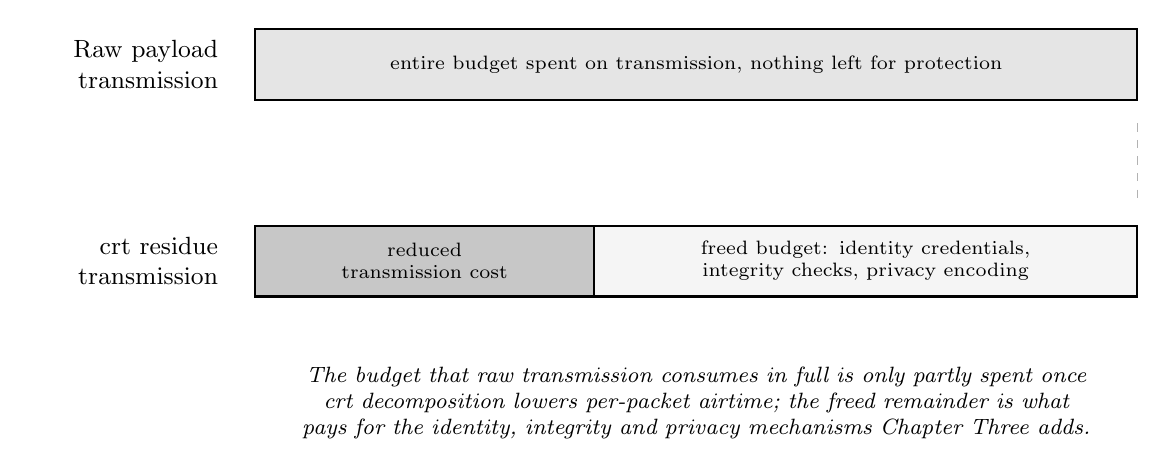
\begin{tikzpicture}[
      barlabel/.style={font=\small, align=right, anchor=east, text width=23mm},
      seglabel/.style={font=\scriptsize, align=center},
      note/.style={font=\footnotesize\itshape, align=center, text width=105mm}
    ]
    \def\barw{11.2}
    \def\barh{0.9}

    \node[barlabel] at (-0.35,3) {Raw payload\\transmission};
    \draw[thick, fill=black!10] (0,3-\barh/2) rectangle (\barw,3+\barh/2);
    \node[seglabel, text width=88mm] at (\barw/2,3)
      {entire budget spent on transmission, nothing left for protection};

    \node[barlabel] at (-0.35,0.5) {\gls{crt} residue\\transmission};
    \draw[thick, fill=black!22] (0,0.5-\barh/2) rectangle (4.3,0.5+\barh/2);
    \draw[thick, fill=black!4] (4.3,0.5-\barh/2) rectangle (\barw,0.5+\barh/2);
    \node[seglabel, text width=34mm] at (2.15,0.5) {reduced\\transmission cost};
    \node[seglabel, text width=58mm] at (7.75,0.5)
      {freed budget: identity credentials, integrity checks, privacy encoding};

    \draw[dashed, gray!60] (\barw,3-\barh/2-0.3) -- (\barw,0.5+\barh/2+0.3);

    \node[note] at (\barw/2,-1.3)
      {The budget that raw transmission consumes in full is only partly spent
       once \gls{crt} decomposition lowers per-packet airtime; the freed
       remainder is what pays for the identity, integrity and privacy
       mechanisms Chapter Three adds.};
  \end{tikzpicture}
  \caption{Reallocating the transmission budget: airtime saved by residue
           decomposition funds identity, integrity and privacy protection.}
  \label{fig:budget-reallocation}
\end{figure}

The two mechanisms also compose cleanly. Residue
decomposition and ledger verification operate on the same object at different
points in its life, the first on the reading in flight and the second on the
record at rest, and the quantity each is sensitive to is different: the radio
cares about occupancy, the ledger about the size and count of committed
transactions. A scheme that reduces occupancy without increasing transaction
count therefore improves one without taxing the other, which is not generally
true of protection mechanisms and is worth demonstrating rather than assuming.

There is also an evidential gap. Claims about edge blockchain feasibility are
typically supported by simulation or short laboratory runs. A
sustained field deployment on real hardware, through real weather and real
connectivity failures, produces a different and more useful class of evidence,
including the failure modes that simulation does not generate.

The applied case is direct. Smallholder and arid-region agriculture is where
both the water-efficiency gains and the certification-fraud exposure are
largest, and where infrastructure assumptions of existing systems are least
likely to hold.

\section{Objectives of the Study}
\label{sec:objectives}

\subsection{Main Objective}
\label{subsec:main_objective}

\textbf{To design, implement and evaluate a distributed blockchain-based
framework that protects identity, integrity and privacy in agricultural data
processing, and to validate it in a sustained field deployment on constrained
edge hardware.}

\subsection{Specific Objectives}
\label{subsec:specific_objectives}

\begin{enumerate}
  \item \textbf{Analyse} the identity, integrity and privacy requirements of
        agricultural data pipelines, decomposing the threat surface from
        sensing node through gateway to ledger into an attacker model with
        stated capabilities and assumptions.

  \item \textbf{Design} an integrated protection scheme combining \gls{crt}
        multi-channel residue transmission, which lowers per-packet airtime
        while preserving exact reconstruction, with an identity layer that
        binds each reading to an authenticated originating node through
        \gls{hlf} \gls{msp} credentials and \gls{hrbac} policy enforced in
        chaincode.

  \item \textbf{Implement} the framework on a heterogeneous edge cluster of
        \gls{esp32} sensing nodes and \gls{arm64} \gls{rpi} gateways running
        \gls{hlf} under Raft ordering, deployed under real agricultural
        operating conditions.

  \item \textbf{Evaluate} the transmission, ledger and access-control layers
        against compression and centralised baselines on airtime, energy,
        throughput, latency and memory footprint, and assess the scalability
        and fault-tolerance envelope through queuing-theoretic analysis
        validated against measured load.
\end{enumerate}

\section{Research Questions}
\label{sec:research_questions}

\begin{enumerate}[label=\textbf{RQ\arabic*.}]
  \item To what extent can \gls{crt} residue decomposition reduce per-packet
        airtime and increase gateway packet capacity without loss of
        reconstruction fidelity?
  \item Can a permissioned distributed ledger sustain the throughput and latency
        required by real-time irrigation control when hosted entirely on
        \gls{arm64} edge gateways?
  \item What identity binding is required for a ledger record to attest to the
        originating sensing node rather than merely to the submitting gateway,
        and what does that binding cost?
  \item What confidentiality is obtained by distributing residues across
        channels and custodians, and under what adversary model does it hold?
  \item How does the integrated framework behave as offered load approaches
        gateway and ledger saturation, and where are its practical limits?
\end{enumerate}

\section{Research Hypotheses}
\label{sec:hypotheses}

\begin{description}
  \item[\textnormal{\textbf{H1 (Transmission efficiency).}}] \gls{crt} residue
        transmission reduces per-packet airtime by at least 40\% relative to raw
        transmission while maintaining at least 99\% reconstruction accuracy.

  \item[\textnormal{\textbf{H2 (Edge ledger performance).}}] \gls{hlf} hosted on
        four \gls{rpi} 4B gateways sustains a mean transaction latency below
        \SI{2}{\second} at an average throughput of at least \SI{50}{\tps}.

  \item[\textnormal{\textbf{H3 (Access-control overhead).}}] Enforcing
        \gls{rbac} in chaincode preserves at least \SI{50}{\tps} and keeps mean
        smart-contract execution below \SI{500}{\milli\second}.

  \item[\textnormal{\textbf{H4 (Field robustness).}}] Sustained field operation
        maintains at least 99\% end-to-end reliability, with measured airtime
        within \SI{5}{\milli\second} of the analytical model.

  \item[\textnormal{\textbf{H5 (Privacy preservation).}}] An adversary observing
        fewer than $k$ of the $k$ residue channels cannot reconstruct the
        original reading, and the residual information leakage remains below a
        stated bound.
\end{description}

%% VERIFY: H5 is new to the thesis and is not yet supported by the source
%% article. It requires either a formal argument or an empirical leakage
%% measurement before Chapter Four is written. Tracked in JOURNAL.md.

\section{Scope and Delimitations}
\label{sec:scope}

\textbf{In scope.} Sub-GHz \gls{lora} sensing networks of the order of fifty
nodes; permissioned ledgers of the \gls{hlf} family under Raft ordering;
gateway hardware in the \gls{rpi} 4B class; agronomic telemetry, specifically
soil moisture, temperature, humidity and irrigation actuation; and the
identity, integrity and privacy properties of that pipeline.

\textbf{Out of scope.} Public permissionless blockchains and their consensus
economics; cellular and satellite backhaul; image-based and remote-sensing
agronomy; agronomic model accuracy as such, which is treated as given rather
than as an object of study; and formal cryptographic proofs of the underlying
primitives, which are cited rather than re-derived.

\textbf{Delimitations.} Field validation is drawn from a single deployment site
and a single cropping season, which bounds the claims that can be made about
generalisation across soil types and climates. Node population is bounded by
what could be instrumented. Behaviour beyond that population is established
analytically and by synthetic load rather than by direct measurement.

\section{Significance of the Study}
\label{sec:significance}

For \textbf{engineering practice}, the work supplies measured rather than
simulated evidence about what a permissioned ledger costs on edge hardware, and
a transmission scheme that reduces that cost enough to make protection
affordable.

For \textbf{the research literature}, it connects two bodies of work that have
developed separately, namely residue arithmetic for communication efficiency and
distributed ledgers for data provenance, and shows that the first can subsidise
the second.

\textbf{Methodologically}, the work contributes a characterisation obtained under
field conditions rather than in a laboratory. Failures that a testbed does not
generate, mesh partitions, thermal derating, intermittent backhaul and the
recovery behaviour that follows each, are exactly the ones that determine
whether such a system is deployable, and they only appear when the system is
left running.

For \textbf{agricultural stakeholders}, it offers a path to verifiable
certification and insurance records that does not require farmers to surrender
commercially sensitive detail to every consortium member.

\section{Definition of Key Terms}
\label{sec:definitions}

\begin{description}
  \item[Airtime] The time a radio occupies a channel to transmit one packet. It
        governs both node energy consumption and gateway capacity.

  \item[Residue] The remainder of a reading modulo one of a set of pairwise
        coprime moduli. A complete residue set uniquely determines the original
        value below the product of the moduli.

  \item[Integrity] The property that a record has not been altered since it was
        committed, and that alteration would be detectable.

  \item[Identity] The property that a record can be attributed to a specific
        authenticated principal, here a specific sensing node rather than
        merely a gateway.

  \item[Privacy] The property that a record's content is disclosed only to
        principals authorised to see it, notwithstanding replication of the
        ledger.

  \item[Endorsement] In \gls{hlf}, the process by which designated peers
        simulate a transaction and sign the result before ordering.
\end{description}

\section{Organisation of the Thesis}
\label{sec:organisation}

\textbf{Chapter One} states the background, problem, rationale, objectives,
questions and hypotheses. \textbf{Chapter Two} reviews the literature on
precision agriculture and \gls{iot} sensing, transmission optimisation,
distributed ledgers in agriculture, edge-resident consensus and
privacy-preserving data processing, and identifies the gap this work addresses.
\textbf{Chapter Three} presents the materials and methods: system architecture,
\gls{crt} formulation, identity and access-control design, hardware
implementation, deployment protocol and evaluation methodology.
\textbf{Chapter Four} reports results and applications across the transmission,
ledger, access-control and agricultural-outcome dimensions. \textbf{Chapter
Five} discusses the findings against the hypotheses, states limitations and
threats to validity, and sets out conclusions, recommendations and perspectives
for further research.
